\chapter{Implementation in Unity Engine}
This chapter describes how the theoretical model described in the previous chapters has been implemented in practice, detailing the specific parameters defined previously.

In addition, due to its technical nature, the nomenclature from Unity engine \cite{UnityGlossary} will be used, in particular:

\begin{description}
    \item[GameObject] - used to represent everything which can exists in scene. Every object in game is GameObject. GameObject contains components.
    \item[Prefab] - The Prefab Asset acts as a template from which new Prefab instances (GameObjects) can be created in the Scene
    \item[Component] - object that define properties and behaviour of GameObject it is attached to.
\end{description}
Project and the source code can be found in public repository on GitHub:
\url{https://github.com/kerdamon/Engineering-Thesis-Simulating-Ecosystem}

\section{Components}
Below is the list of custom components written for the project:

\begin{enumerate}
    \item State machine - handling state change described in \autoref{switchingStates}
    \item Interactions - handling interactions described in \autoref{interactionDescription}
    \item Interaction managers - handling the initiation of the corresponding interaction when an agent wants to initiate it and the appropriate conditions are met
    \item Agent component - handling training and inference of ML model
    \item Simulation Control - gathering statistics during simulation
    \item Training Area managers - controlling training environment, for example, provides the ability to place agents in a random position in a training environment
    \item Food managing - components used to control plant growth
    \item Needs - managing needs of agent
    \item Features - managing features of agent
\end{enumerate}
As the thesis does not focus on a strictly technical approach to the problem, it is not necessary to describe most of the components, except for the description interactions and values of parameters for features, needs and sates in order to make their functioning more precise.

\subsection{Interactions}
\label{interactionsImplementationDescription}
Below are specific values of parameters regulating the functioning of the interactions defined in \autoref{interactionDescription}

\subsubsection{Drinking Interaction}
\begin{description}
    \item[Max drinking time] - after this time agent regenerates max thirst: 10 s
    \item[Step time] - determines the minimum time to record drinking progress: 0.5s
    \item[Regeneration per step] - amount by which thirst changes in each step: 5
\end{description}

\subsubsection{Mating Interaction}
\begin{description}
    \item[Duration time]: 5 s
\end{description}

\subsubsection{Eating Carrot Interaction}
\begin{description}
    \item[Max eating time] - after this time agent regenerates max hunger: 10 s
    \item[Step time] - determines the minimum time to record eating progress: 1s
    \item[Regeneration per step] - amount by which hunger changes in each step: 10
\end{description}

% \subsection{Features}
% \label{featuresImplementationDescription}
% Below are the specific values of the parameters described in the definition of features in \autoref{featuresDefinition}
% \begin{description}
%     \item[Speed] $a_s = 1$
%     \item[Sensory range] $r_{min} = 15, r_{max} = 27$
%     \item[Fertility] $d = 3$
% \end{description}

% \subsection{Needs}
% \label{needsImplementationDescription}
% Below are the specific values of the parameters described in the definition of needs in \autoref{needsDefinition}
% \begin{description}
%     \item[Growth rate] $\alpha = 0.5$
% \end{description}

% \subsection{States}
% \label{statesImplementationDescription}
% Below are the specific values of the parameters described in the definition of the states in \autoref{statesDefinition}
% \begin{description}
%     \item[Chilling] $a_c = 0.6$
%     \item[Looking for mate] $a_m = 1.01$
% \end{description}

\subsection{Features, needs and states}
\label{featuresNeedsStatesImplementation}
Below are the specific values of the parameters described in the definition of features, needs and states (subsections \ref{featuresDefinition}, \ref{needsDefinition} and \ref{statesDefinition}).
\begin{center}
    \begin{tabular}{ |c|c|c| } 
        \hline
        Name & Symbol & Value \\
        \hline \hline
        Speed coefficient & $a_s$ & 1 \\
        \hline
        Minimal sensory range & $r_{min}$ & 15 \\
        \hline
        Maximal sensory range & $r_{max}$ & 27 \\ 
        \hline
        Offspring variation by feature & $d$ & Rabbits: 3 \\
        &  & Foxes: 2 \\ 
        \hline
        Growth rate & $\alpha$ & 0.5 \\ 
        \hline
        Chilling coefficient & $a_c$ & 0.6 \\ 
        \hline
        Mating coefficient & $a_m$ & 1.01 \\ 
        \hline
    \end{tabular}
\end{center}



\section{Prefabs}
\subsubsection{Simulation and training Areas}
Areas contain agents together with environment. Each area contains terrain - plane, boundaries, water, food generators, rabbits and predators.

\begin{figure}
    \centering
    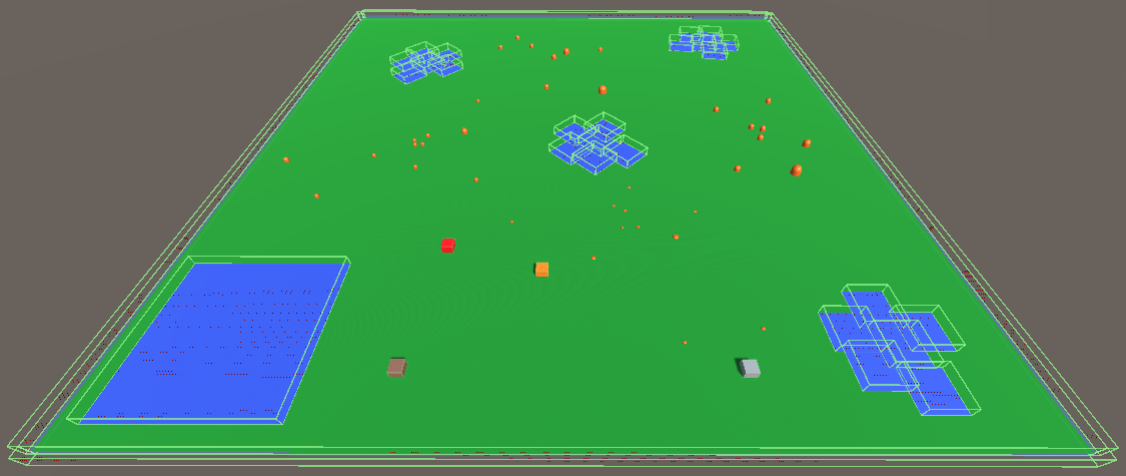
\includegraphics[width=\textwidth]{Images/simulation_area.png}
    \caption{Simulation area in Unity editor.}
    \label{fig:simulationArea}
\end{figure}

\subsubsection{Agents}
An agent is just an implementation of the agent defined in \autoref{agentsChapter}. 
The agent's body is a cube with side length 1. The agent also has a cubic collider which is used to initiate interactions with side length $1.5$, so it does not need to directly touch the body of the object it wants to interact with. 

Precision grid sensor has dimensions of 37 x 40 and a cell size of 1.5. Long-range grid sensor has dimensions of 20 x 20 and a cell size of $40$. The sensor has such a large range because, due to technical limitations, the smallest possible size of this sensor is 20x20, and the cell size had to be chosen so as not to give the agent the exact position of the object, only its general location.

The rabbit can give birth to a base of 6 offspring, the discrepancy due to fecundity is 3, while randomness can modify the number of offspring by 2. Thus, the final number of offspring the rabbit can give birth to is 1-11. For the fox, these numbers are 4, 2, and 1, respectively, giving a final number of offspring of 1 - 7. The probability of mutation is 0.005.

\subsubsection{Plant Generator and Carrots}
The carrot is a capsule of size 1, although it is modified according to the growth level of the plant. Its minimum size is 0.5, maximum is 1.5, and during growth it changes by 0.1 every 5 seconds. For the Plant Generator, the spawn range is 8, the spawn radius is equal to 6, and the plant limit is 15, but these parameters may vary depending on the simulation.

\subsubsection{Water}
Water is just a plane with a collider placed above its surface to allow sensors to detect it and to prevent agents from moving through the water. The base size of the water element is 5x5, while the sea element is 20x20. The lake element consists of 6 merged water elements.

\section{Scenes}
The project was divided into 6 scenes. Five of them are training scenes and one is a simulation scene. The training scenes are slightly modified versions of the simulation scene for purposes of training ML models. Each training scene contains multiple training areas specific to each model in order to train it better and faster. The base size of the plane is 200x200. 

Each scene contain main camera, lighting, event system (used for inputting keys) and area with environment and agents.

\subsubsection{Simulation scene layout}
Area present in this scene contains agents with with normal setup and behaviour with all states, models and interactions defined in \autoref{ecosystemDefinitionChapter} and \autoref{agentsChapter} and further specified above in this chapter.
Simulation scene also includes simulation controller GameObject responsible for measuring statistics during simulations and logging it, as well as canvas GameObject for displaying it on screen.

\subsubsection{Training scene layout}
The area present in this scene contains agents with modified states, interactions and simplified behaviours tailored to the specific model being trained. For example, in the mating training scene, the agents use a simplified mating interaction in which the male only needs to find a female and interact with her, after which the female is moved to a new random position and the male continues to search for a mate. There are also several copies of areas in the scenes to speed up the training of the model.

\begin{figure}
    \centering
    \includegraphics{Images/scene_layout_combined.png}
    \caption{Simulation and training scene layouts.}
    \label{fig:sceneLayout}
\end{figure}

The individual training scenes are described in more detail in \autoref{trainingEnvironmentsDescription}